\documentclass[landscape,aspectratio=169]{slides}
%\usepackage{standard-slide-include}
\usepackage{color, amsmath}
\usepackage{physics}
\usepackage{shadow}     % this creates a shaded box; see \shabox below
\usepackage{physics}
\usepackage{amsmath}
\usepackage{amssymb}
\usepackage{amsmath}
\usepackage{graphicx}
\usepackage{amsthm, mathtools}
%\usepackage{hyperref}
\usepackage{color}
\title{\textcolor{blue}{\textbf{Tensor Algebra}}}
\date{September 10, 2020}
\author{Aditya Vijaykumar}

\definecolor{dark-magenta}{rgb}{.5,0,.5}
\definecolor{myblack}{rgb}{0,0,0}
\definecolor{darkgray}{gray}{0.5}
\definecolor{lightgray}{gray}{0.75}

\begin{document}
	\maketitle
	\begin{slide}
	
	Newtonian equations of motion are often phrased in the language of vectors.
	
	For example, 	
	\begin{equation}\label{key}
	\va{F}_{12} = - G \dfrac{m_1 m_2}{\abs{\va{r}}^3} \va{r}  \qq{.}
	\end{equation}
	Here, $ \va{F}_{12} $ is the force on $ m_2 $ due to $ m_1 $. There are two ways of looking at this equation:
	\begin{itemize}
		\item A \textit{coordinate-free way}
		\item A \textit{coordinate-dependent way}
	\end{itemize}
	Similarly,  relativistic equations are phrased in the language of tensors.
\end{slide}
\begin{slide}
	\textcolor{blue}{\textbf{Manifolds}}
	
	A tensor is a geometrical object defined on a \textit{manifold}.
	
	A manifold in $ n $-dimensions is something that \textit{locally} looks like $ n $-dimensional Euclidean (flat) space $\mathbb{R}^n $, \textit{eg.} $ S^2 $ or even the Earth!
	
	A manifold is then simply a set of points such that each point possesses a set of $ n $-coordinates $ (x^1, x^2, \ldots, x^n) $ which are all real numbers.
\end{slide}	
\begin{slide}
	To add to this, it might even be impossible to cover a manifold in full by a non-degenerate coordinate system.
	
	\textit{Euclidean Example}: Plane polar coordinates have a degeneracy at the origin where $ \phi $ becomes indeterminate; we could make do with Cartesian coordinates in this case though.
	
	\textit{But}: There is no coordinate system that covers the whole of $ S^2 $ without degeneracy. 

\end{slide}

\begin{slide}
	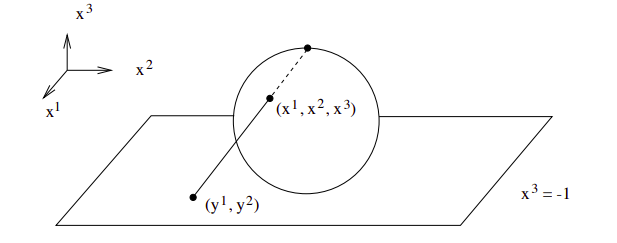
\includegraphics{images/stereograph.png}
	\centering{\textit{Source}: Sean Carroll's GR Lecture Notes}

	Often, it is convenient to work with only one of these coordinate systems (called \textit{coordinate patch}) and keep track of the points that aren't included.
\end{slide}
\begin{slide}	
	\textcolor{blue}{\textbf{Curves and Surfaces}}
	
	Interested in the subset of points that form curves and surfaces.
	
	We shall often define them parametrically. For example, since a curve has one degree of freedom, it will depend only on one \textit{parameter}; we can define it by:
	\begin{equation}\label{key}
	x^a = x^a(u) \qq{,}
	\end{equation}
	where $ u $ is the parameter and $ x^1(u), x^2(u), \ldots, x^n(u) $ are all functions of $ u $.
	
	Similarly, since a surface of $ m $ dimensions will have $m$ degrees of freedom, we can define it by a set of $ m $ parameters:
	\begin{equation}\label{key}
	x^a = x^a(u^1, u^2, \ldots, u^m) \qq{.}
	\end{equation}
\end{slide}	
\begin{slide}
	In particular, if $ m=n-1 $, the surface is called a \textit{hypersurface}. 
	
	Here, one can eliminate $ n-1 $ parameters from $ n $ equations to give one equation connecting the coordinates \textit{ie.},
	\begin{equation}\label{hyp}
	f(x^1, x^2, \ldots, x^n) = 0 \qq{.}
	\end{equation}
	
	Equivalently, if a point on an $ n $-dimensional manifold is constrained to lie on a hypersurface, it should follow eq. \ref{hyp}. Similarly, points on an $ m $-dimensional surface should follow $ n-m $ such constraints.
\end{slide}

\begin{slide}
	\textcolor{blue}{\textbf{Transformation of Coordinates}}
	
	Let's consider a transformation of coordinates $ x^a $ to $$ x'^a =  f^a (x_1, x_2,\ldots, x_n) $$ where $ f^a $'s are single-valued.
	
	$ \implies $ Passively assigning a point with coordinates $ (x^1, x^2,\ldots, x^n) $ the new coordinates $ (x'^1,x'^2, \ldots, x'^n) $. 
	
	$ \implies $More succintly, we will just use the notation $ x'^a = x'^a(x) $
	
	What will the transformation look like?

\end{slide}	

\begin{slide}
	We differentiate $ x' $ with respect to $ x $ $ \implies $ a matrix of coefficients:
	\begin{equation}\label{jaco}
	\mqty[\pdv{x'^a}{x^b}] = \mqty[\pdv{x'^1}{x^1} & \pdv{x'^1}{x^2} & \ldots & \pdv{x'^1}{x^n} \\
	\pdv{x'^2}{x^1} & \pdv{x'^2}{x^2} & \ldots & \pdv{x'^2}{x^n} \\
	\vdots & & & \\
	\pdv{x'^n}{x^1} & \pdv{x'^n}{x^2} & \ldots & \pdv{x'^n}{x^n} 
	]
	\end{equation}

The determinant of the above transformation matrix is called the Jacobian $ J' $ of the transformation.

If $ J' $ is non-zero, we can solve eq \ref{jaco} and find the inverse transformation $ x^a = x^a(x') $. 

Using the product rule of determinants, the Jacobian of the inverse transformation $ J = 1/J'$
\end{slide}

\begin{slide}
	How would the total differential of $ x'^a $ relate to the transformation matrix?\begin{equation}\label{difftransform}
	\dd{x'^a} = \sum_{b = 1}^{n} \pdv{x'^a}{x^b} \dd{x^b} = \pdv{x'^a}{x^b} \dd{x^b}  \qq{,}
	\end{equation}
	
	We invoke the \textit{Einstein summation convention} to simplify our equations.
	
	We drop the summation sign altogether and understand that whenever an index is repeated in, it should be summed over.
	
	This repeated index is also often called the \textit{bound index} or the \textit{dummy index}.
	
	
\end{slide}

\begin{slide}
	\textit{Aside}: The \textit{Kronecker delta} is a quantity which is either $ 0 $ or $ 1 $ according to
	\begin{equation}\label{key}
	\delta^a_b = \begin{cases}
	1 \qq{if} a = b\\
	0 \qq{if} a \ne b
	\end{cases} \implies \pdv{x^a}{x^b} = \pdv{x'^a}{x'^b} = \delta^a_b \qq{.}
	\end{equation}
\end{slide}

\begin{slide}
	\textcolor{blue}{\textbf{Contravariant Tensor}}
	
	Let's first define a contravariant vector.
	
	Consider two neighbouring points on a manifold $ P $ and $ Q $ with coordinates $ x^a $ and $ x^a + \dd{x^a} $.
	
	This forms an infinitesimal vector $ \va{PQ} $ attached at $ P $ and directed to $ Q $, whose components in this coordinate system are $ \dd{x^a} $. 
	
	This vector will get transformed to $ \dd{x'^a} $ in the new coordinate system as we have seen. Note that the transformation matrix in this case will be evaluated at point $ P $.
\end{slide}

\begin{slide}
	We then define a \textit{contravariant vector} $ X^a $ as a set of of quantities associated with point $ P $ which transform under a change of coordinates according to
	\begin{equation}\label{key}
	X'^a = \pdv{x'^a}{x^b} X^b \qq{,}
	\end{equation}
	with the transformation matrix evaluated at $ P $.
	
	This definition of the contravariant vector can then be generalized to \textit{contravariant tensors}. 
\end{slide}

\begin{slide}

	A contravariant tensor of rank $ m $ in $ n $-dimensions is a set of $ n^m $ quantities associated with a point $ P $ that follow (for $ m=2 $)
	\begin{equation}\label{key}
	X'^{ab} =  \pdv{x'^a}{x^c}  \pdv{x'^b}{x^d} X^{cd} \qq{.}
	\end{equation}
	
	The transformation properties of higher rank tensors can be obtained in an analogous manner. 
	
	\textit{Special Case}: tensor of rank zero -- which is basically a scalar! This transforms according to $ \phi' = \phi $.
\end{slide}

\begin{slide}
	\textcolor{blue}{\textbf{Covariant and Mixed Tensors}}
	
	Consider a real, continuous, differentiable scalar $ \phi = \phi(x) $. Differentiate $ \phi $ with respect to $ x'^a $,
	\begin{equation}\label{key}
	\pdv{\phi}{x'^a} = \pdv{\phi}{x^b} \pdv{x^b}{x'^a} \qq{.}
	\end{equation}
	
	Note that this involves the inverse tranformation from a coordinate system $ x' $ to $ x $.
	\begin{equation}\label{key}
	 \qq{Hence covariant vector:}X'_a = \pdv{x^b}{x'^a} X_b \qq{,}
	\end{equation}
\end{slide}

\begin{slide}
	\begin{equation*}\label{key}
	\qq{Analogously, rank $ 2 $ covariant tensor:} X'_{ab} = \pdv{x^c}{x'^b} \pdv{x^d}{x'^c} X_{cd} \qq{,}
	\end{equation*}
	and so on for higher rank tensors. In the same spirit, we can define  by the law
	\begin{equation*}\label{key}
	\qq{Mixed tensors of rank 3:}
	X'^{a}_{bc} =  \pdv{x'^a}{x^d} \pdv{x^e}{x'^b} \pdv{x^f}{x'^c} X^d_{ef} \qq{.} 
	\end{equation*}
	
	If a mixed tensor has contravariant rank $ p $ and covariant rank $ q $, it is said to have \textit{type}  or \textit{valence} $ (p,q) $.
\end{slide}

\begin{slide}	
	Let's say we find two tensors $ X_{ab} $ and $ Y_{ab} $ which are equal component-by-component in a certain coordinate system \textit{ie.} $$ X_{ab} = Y_{ab} $$Will the tensors still be equal in a transformed coordinate system? Yes! Multiply on both sides by transformation matrix.

	We might be interested in introducing coordinate systems for the purposes of a specific problem, but tensorial equations are essentially coordinate-independent.
	
\end{slide}

\begin{slide}
	\textcolor{blue}{\textbf{Tensor Fields}}
	
	In vector analysis, a \textit{vector field} defined in a region is the association of a vector to every point in that region.
	
	Analogously, a tensor field defined in a region is the association of a tensor with the same valence to every point in the region; \textit{ie},
	\begin{equation*}\label{key}
	P \rightarrow T^{a \ldots}_{b\ldots} (P) \qq{,}
	\end{equation*}
	where $  T^{a \ldots}_{b\ldots} (P) $ is the value of the tensor at $ P $.
	
	The tensor field is called continuous and differentiable if its coordinates are continuous and differentiable functions. 
	
	The tensor field is called smooth is its components are differentiable to all orders, denoted mathematically by saying that the components are $ C^\infty $.
	
\end{slide}

\begin{slide}
	\textcolor{blue}{\textbf{Some Elementary Operations}}
	
	\begin{itemize}
		\item $X^a_{bc} = Y^a_{bc} + Z^a_{bc}$
		\item $ X^a_{bc} = \alpha W^a_{bc} $, where $ \alpha $ is a scalar.
		\item A covariant tensor of rank $ 2 $,  $ X_{ab} $, is said to be symmetric if $ X_{ab} = X_{ba} $. In this case, it has $ \frac{n(n+1)}{2} $ independent components.
		\item A covariant tensor of rank $ 2 $,  $ X_{ab} $, is said to be anti-symmetric if $ X_{ab} = -X_{ba} $. In this case, it has $ \frac{n(n-1)}{2} $ independent components.
		\item Given a covariant tensor of rank $ 2 $, one can write it as a sum of a symmetric tensor and an anti-symmetric tensor,
		\begin{align*}
		X_{ab} = &X_{(ab)} + X_{[ab]} \qq{,} \\
		\qq{where} X_{(ab)} = \dfrac{X_{ab} + X_{ba}}{2} &\qq{and} X_{[ab]} = \dfrac{X_{ab} - X_{ba}}{2} \qq{.}
		\end{align*}
	\end{itemize}

\end{slide}
\begin{slide}
	\begin{itemize}	
		\item In general,
		\begin{align*}
		X_{(a_1 a_2 \ldots a_r)} &= \dfrac{1}{r!} \text{(sum over all permutations of indices)} \\
		X_{[a_1 a_2 \ldots a_r]} &= \dfrac{1}{r!} \text{(alternating sum over all permutations of indices)} 	\qq{.}	
		\end{align*}
		
		For example, 
		\begin{equation*}\label{key}
		X_{[abc] }  = \dfrac{1}{6!} \qty(X_{abc} -X_{acb} + X_{cab} - X_{cba} + X_{bca} - X_{bac}) \qq{.}
		\end{equation*}
		\item We can multiply a type $ (p_1, q_1) $ tensor and a type $ (p_2, q_2) $ tensor to get a type $ (p_1+p_2, q_1+q_2) $ tensor, \textit{eg.} $ X^a_{bcd}  = Y^a_b Z_{cd}$
	\end{itemize}
\end{slide}
\begin{slide}
	\begin{itemize}
		\item Given a tensor of type $ (p,q) $, we can construct a type $ (p-1, q-1) $ tensor by the process of contraction \textit{ie} said a raised index equal to the lower index,
		$$ X^{a}_{bcd} \rightarrow_{contraction}  X^{a}_{acd}  = \delta_a^b X^{a}_{acd} = Y_{cd}$$
	\end{itemize}
\end{slide}

\begin{slide}
	\textcolor{blue}{\textbf{Index-free interpretation of covariant tensor fields}}
	
	Let's introduce the following notation,
	\begin{equation}\label{key}
	\partial_a = \pdv{x^a} \qq{.}
	\end{equation}
	
	We then define an operator $ X $ as,
	\begin{equation}\label{key}
	X = X^a \partial_a \implies Xf = X^a \partial_a f = X^a (\partial_a f) \qq{,}
	\end{equation}
	where $ f $ is an arbitrary real-valued function. 
\end{slide}	

\begin{slide}
	The operator $ X $ is does not depend on the choice of the coordinate system $$ X = X^a \pdv{x^a} =X'^a \pdv{x'^a}  $$	
	
	Hence, operating $ X $ on $ f $ will lead to the same result irrespective of the coordinate system used.
	
	Any vector at $ P $ is given by
	\begin{equation}\label{key}
	 X_P = \qty[X^a]_P \qty[\pdv{x^a}]_P
	\end{equation} we can think of the quantities $ [\partial_a]_P $ as forming the basis for all the vectors at $ P $, and $ [X^a]_P $ being the components.
	
	The vector space of all the contravariant vectors at $ P $ is called the \textit{tangent space} at $ P $ and it denoted by $T_P(M)$.
\end{slide}

\begin{slide}
	Given two vector fields $ X $ and $ Y $, we can define a new vector field called the \textit{commutator} or the \textit{Lie bracket} of $ X $ and $ Y $ by
	\begin{equation}\label{key}
	\qty[X, Y] = XY - YX \qq{.}
	\end{equation}
	
	Is the commutator a vector field?
	\begin{align*}
	\qty[X, Y] f &= XYf - YXf \\
	&= X^a \partial_a ( Y^b \partial_b f  ) - Y^b \partial_b (X^a \partial_a ) f \\
	&=\qty(X^a \partial_a Y^b \partial_b    - Y^b \partial_b X^a \partial_a ) f  + \qty(X^a Y^b \partial_a  \partial_b f - Y^b X^a \partial_b \partial_a f) \\
	& = \qty(X^b \partial_b Y^a     - Y^b \partial_b X^a ) \partial_a f \qq{,} 
	\end{align*}
	which proves that $ \qty[X,Y] $ is a vector field.
\end{slide}
\begin{slide}	
	The properties of the Lie bracket are:
	\begin{itemize}
		\item  $ \qty[X,X] = 0 $
		\item $ \comm{X}{Y} = - \comm{Y}{X} $
		\item \textit{Jacobi Identity}: $ \comm{X}{\comm{Y}{Z}} + \comm{Y}{\comm{Z}{X}} + \comm{Z}{\comm{X}{Y}} = 0 $
	\end{itemize}
\end{slide}
\end{document}
